\section{Student-Project Matching Tool}

The SPMT consists of three parts: data collection, the Student Project Matching (SPM) Recommender, and the final set of teams (see Figure \ref{fig:SPM}). Prior to data collection, we needed to first define what skills are currently valued by SWE employers. To do this, we identified six main categories of SWE jobs and searched for them on three popular job-search websites \cite{noauthor_job_nodate-1, noauthor_job_nodate, noauthor_jobs_nodate}. We then selected the first ten job postings for each category on each website and extracted the SWE skills mentioned in their descriptions. Skills that were included in 70\% of a category's job postings were then selected for incorporation into the data collection step of the SPMT. Lastly, the industry partners reviewed the full list of SWE categories and the resulting skills, which are listed in Table \ref{tab:student_skills_survey}.

\begin{table}[t]
    \centering
    \scriptsize
    \begin{tabular}{p{1.5cm}p{1.5cm}p{1.5cm}p{1.5cm}p{1.5cm}p{1.8cm}}
    \hline
        \textbf{Front-end - Web} & \textbf{Front-end - Mobile} & \textbf{Back-end} & \textbf{Databases} & \textbf{ML/AI} & \textbf{Data Science} \\ \hline
        UI/UX & UI/UX & Java & Oracle & Python & Python \\ 
        HTML & Kotlin & PHP & MySQL & OO Lang. & JavaScript \\ 
        CSS & Java & Python & PostreSQL & PyTorch & R \\ 
        Javascript & Swift & C\# & MongoDB & TensorFlow & Tableau \\ 
        React & Unix OS & Ruby & ~ & AWS & Power BI \\ 
        Angular & ~ & REST APIs & ~ & Docker & Spark \\ 
        Vue.js & ~ & TCP/IP & ~ & ~ & Hadoop \\ \hline
    \end{tabular}
    \caption{Skills, tools and frameworks in each SWE category for which students had to rank their level of familiarity in the Student Intake Survey.}
    \label{tab:student_skills_survey}
\end{table}




\subsection{Data Collection}
Data collection was comprised of two student surveys and one project sponsor survey. In the Student Intake Survey, students were asked to indicate their level of confidence in each of the SWE skills listed in Table \ref{tab:student_skills_survey}, as well as which skills they wished to develop or continue improving. In the Sponsor Intake Survey, industry sponsors determined what languages, frameworks, and technologies would be needed for each project. Industry sponsors also submitted 3-minute video project descriptions, and students were asked to rank their interest in each project on the Student Project Ranking Survey. 


\subsubsection{Sponsor Intake Survey}
The Sponsor Intake Survey consisted of 38 questions to learn about the sponsor and their project. Five questions collected sponsor and project information and the mentors' availability to provide technical guidance. The remaining 33 questions asked for the level of relevance of various programming languages, frameworks, and technologies which mapped to the SWE categories in Table \ref{tab:student_skills_survey}.


\subsubsection{Student Intake Survey}

The Student Intake Survey consisted of 72 questions, and its main goal was to understand students' backgrounds and technical goals. Five questions captured students' personal information and demographics. Eight questions captured students' background and goals, focusing on confidence in the field, SWE topic interest, courses taken and grades obtained, and interest in being a team lead. The remaining 59 questions focused on capturing a students' technical background and soft skills. Specifically, the questions focused on students' experience level across a variety of programming languages, frameworks, and technologies. Questions were formatted as single-response multiple-choice, multiple-response multiple-choice, and Likert scales.



\subsubsection{Student Project Ranking Survey}
Industry sponsors were asked to create short video and text summaries of their projects to pitch to students. Students were then asked to fill out the Student Project Ranking Survey, which consisted of 14 questions and the sponsors' video and text descriptions. Students ranked their level of interest for each of the sponsor projects on a 3-point Likert scale (High Interest, Somewhat Interested, No Interest). In the remaining questions, they were able to propose their own project, list potential team members, and express interest in being a team lead.

\begin{figure}
    \centering
    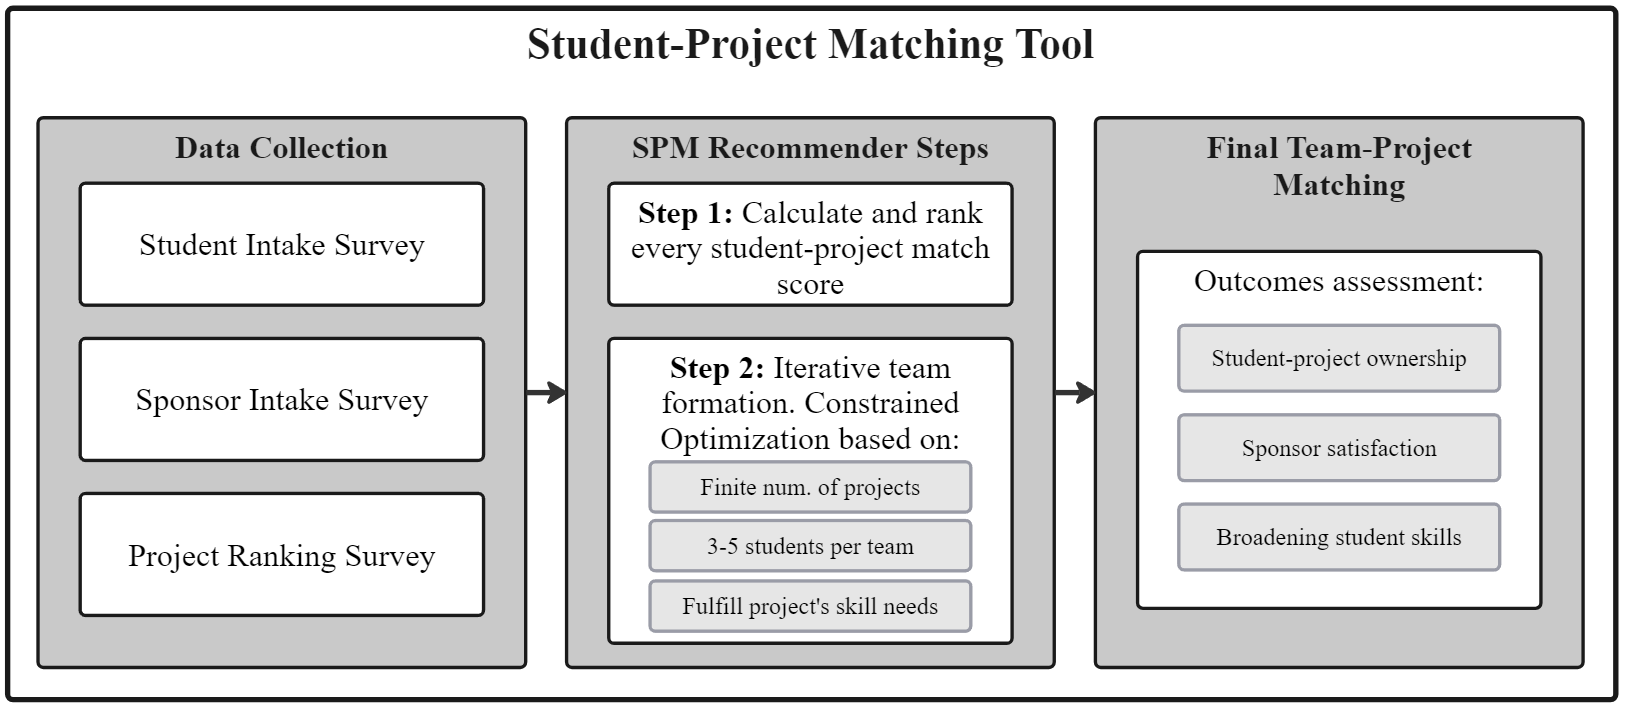
\includegraphics[width=1\linewidth]{Pictures/SPM_Figure.png}
    \caption{Overview of tasks performed by the Student-Project Matching Tool. }
    \label{fig:SPM}
\end{figure}

\subsection{The SPM Recommender}
The SPM Recommender was designed to measure students' fitness and rank them accordingly for each available Sponsor Project by assessing their skills, interests, and knowledge identified through the Intake Surveys. The SPM Recommender was comprised of two steps implemented using Python.

During Step 1, the SPM Recommender imported the responses to the three surveys, iterated through every available industry-sponsored project, and calculated a project score for each student. This score was based on the student's interest and skill levels for each SWE category, and the SWE category's level of relevance for each project. 

In Step 2, student groups were formed and matched while meeting the following constraints (also outlined in Figure \ref{fig:SPM}): Each group must have a maximum of 5 students, only one group can be assigned to each project, there is a finite number of projects (ten for the piloted capstone course), and the project's skill needs must be fulfilled.
These constraints collectively guided the team formation process, striking a balance between individual preferences, project compatibility, and the overall performance potential of each team.

